\subsection{Teorema de Weierstrass}

Un resultado muy importante y ampliamente utilizado se basa en los conceptos anteriores. Este resultado relaciona la existencia de una 
soluci\'on de minimizaci\'on para un problema de optimizaci\'on \cite{no-lineal}. 

\begin{itemize}
   \item Podemos decir que $\overline{x}$ es una soluci\'on de minimizaci\'on al problema $\min \{f(x); x \in S \}$, siempre que 
	 $\overline{x} \in S $ y $ f(\overline{x}) \leqslant f(x)\,\,\,\, \forall \, x \in S$. En tal caso, decimos que existe un m\'inimo.
   \item Por otra parte, decimos que $ \alpha = \inf \{ f(x)| x \in S \} $ si $\alpha $ es la mayor de las cotas inferiores de $ f $ en 
	 $ S; $ estos es: $ \alpha \leqslant f(x) \,\,\, \forall \,\, x\in S $ es decir que no hay $\overline{\alpha} > \alpha$ 
	 tal que $ \overline{\alpha} \leqslant f(x) \,\,\, \forall \, x \in S. $
   \item Similarmente, $\alpha = \max \{ f(x)| x \in S \} $ si existe una soluci\'on $ \overline{x} \in S $ tal que 
	 $\alpha = f(\overline{x}) \geqslant f(x) \,\,\, \forall \, x \in S.$
   \item Por otro lado, $\alpha = \sup \{ f(x)| x \in S \} $ si $ \alpha $ es la menor de las cotas superiores de $ f $ en $ S; $ esto es 
	 $ \alpha \geqslant f(x) \,\,\, \forall \, x \in S, $ y no hay otro $\overline{\alpha} < \alpha $ tal que
	 $ \overline{\alpha} \geqslant f(x) \,\,\, \forall \, x \in S$
\end{itemize}


En la Figura (\ref{no_sol}) se ilustran tres momentos en los que el m\'inimo no existe. \\
En la Figura (\ref{no_sol}a) el \'infimo de de $ f $ sobre $(a, b) $ est\'a dado por $f(b)$ pero como $S$ no es cerrado y en particular
$b \notin S$ el \'inimo no existe.\\
En la Figura (\ref{no_sol}b) tenemos que $\inf \{ f(x);\, x \in [a, b]\} $ es\'a dado por el l\'imite de $f(x)$ cuando x tiende a $b$ por
la izquierda. ($\displaystyle{\lim_{x \rightarrow b^{-}} f(x)}$). Como $f$ es discontinua en $b$ no existe una soluci\'on de minimizaci\'on.\\
La figura (\ref{no_sol}c) ilustra cuando $f $ no es acotada sobre un conjunto $S = \{x: \ x \geqslant a \}$

%------------------------------figura de maximo y minimo-------------------------------

\begin{figure}
   \centering
   \subfigure[$S$ es no cerrado]{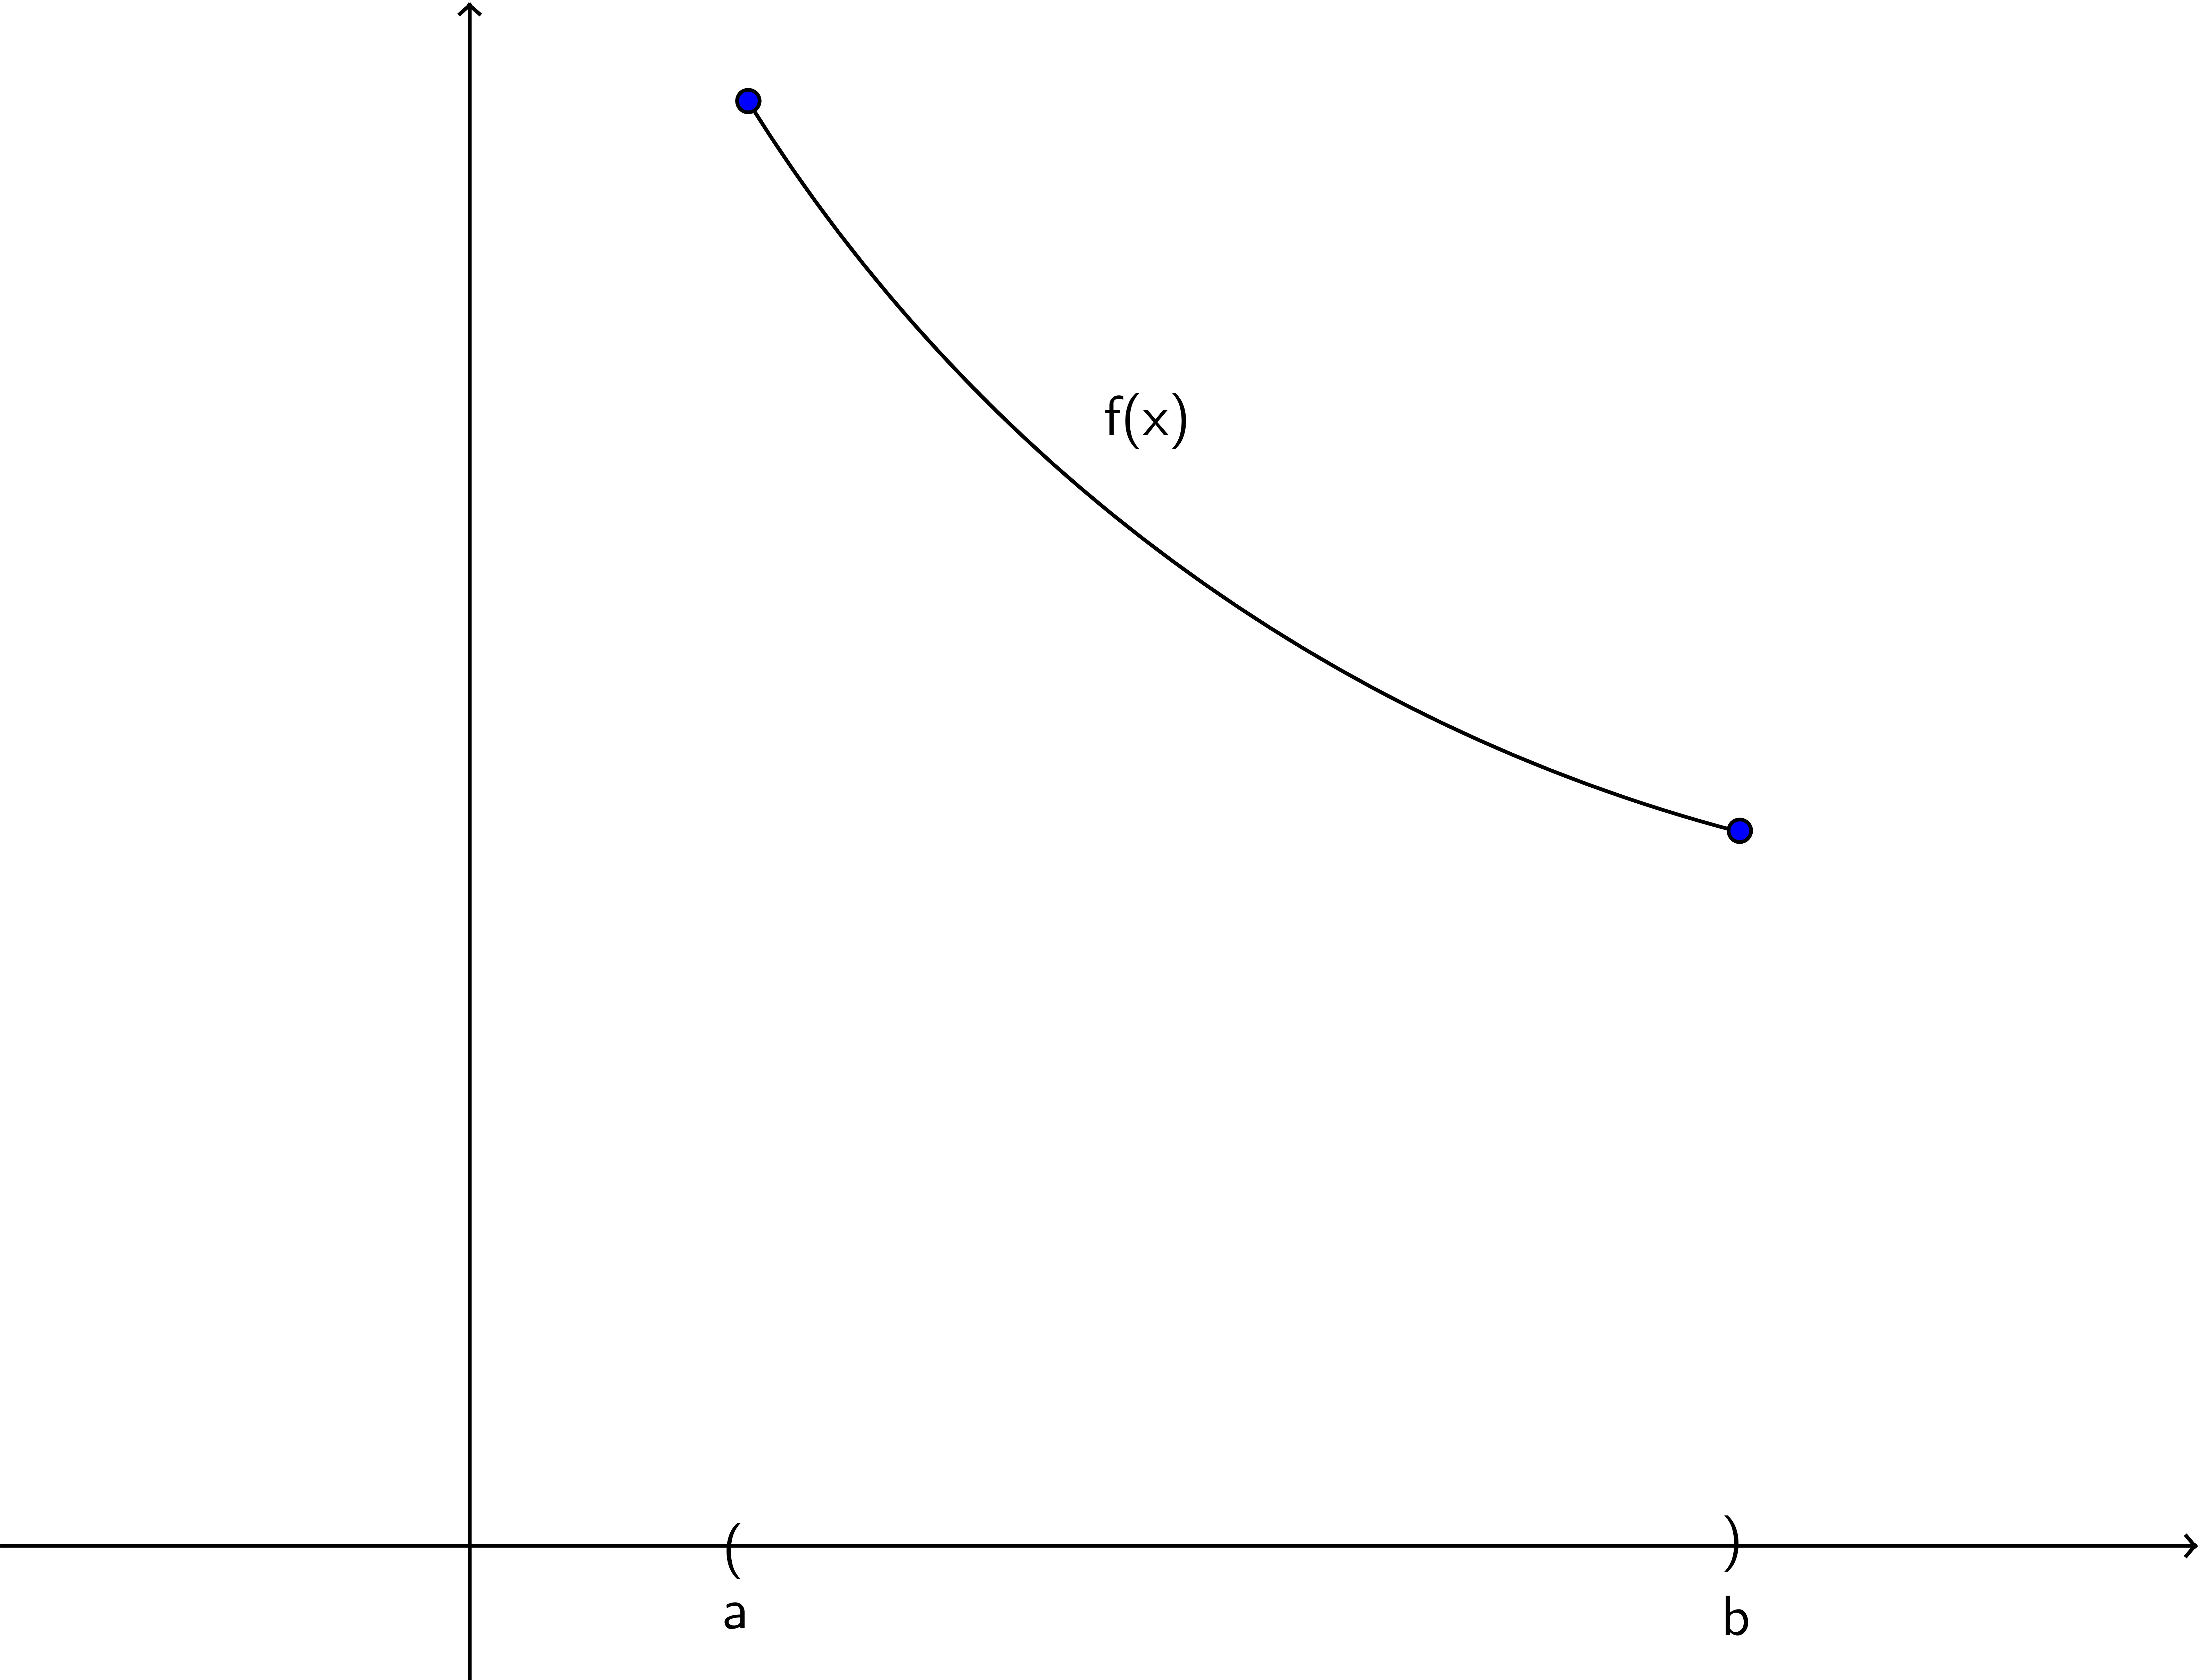
\includegraphics[scale = 0.1]{./partes/sub_sec/2_5a.jpg}}
   \subfigure[$f$ discontinua]{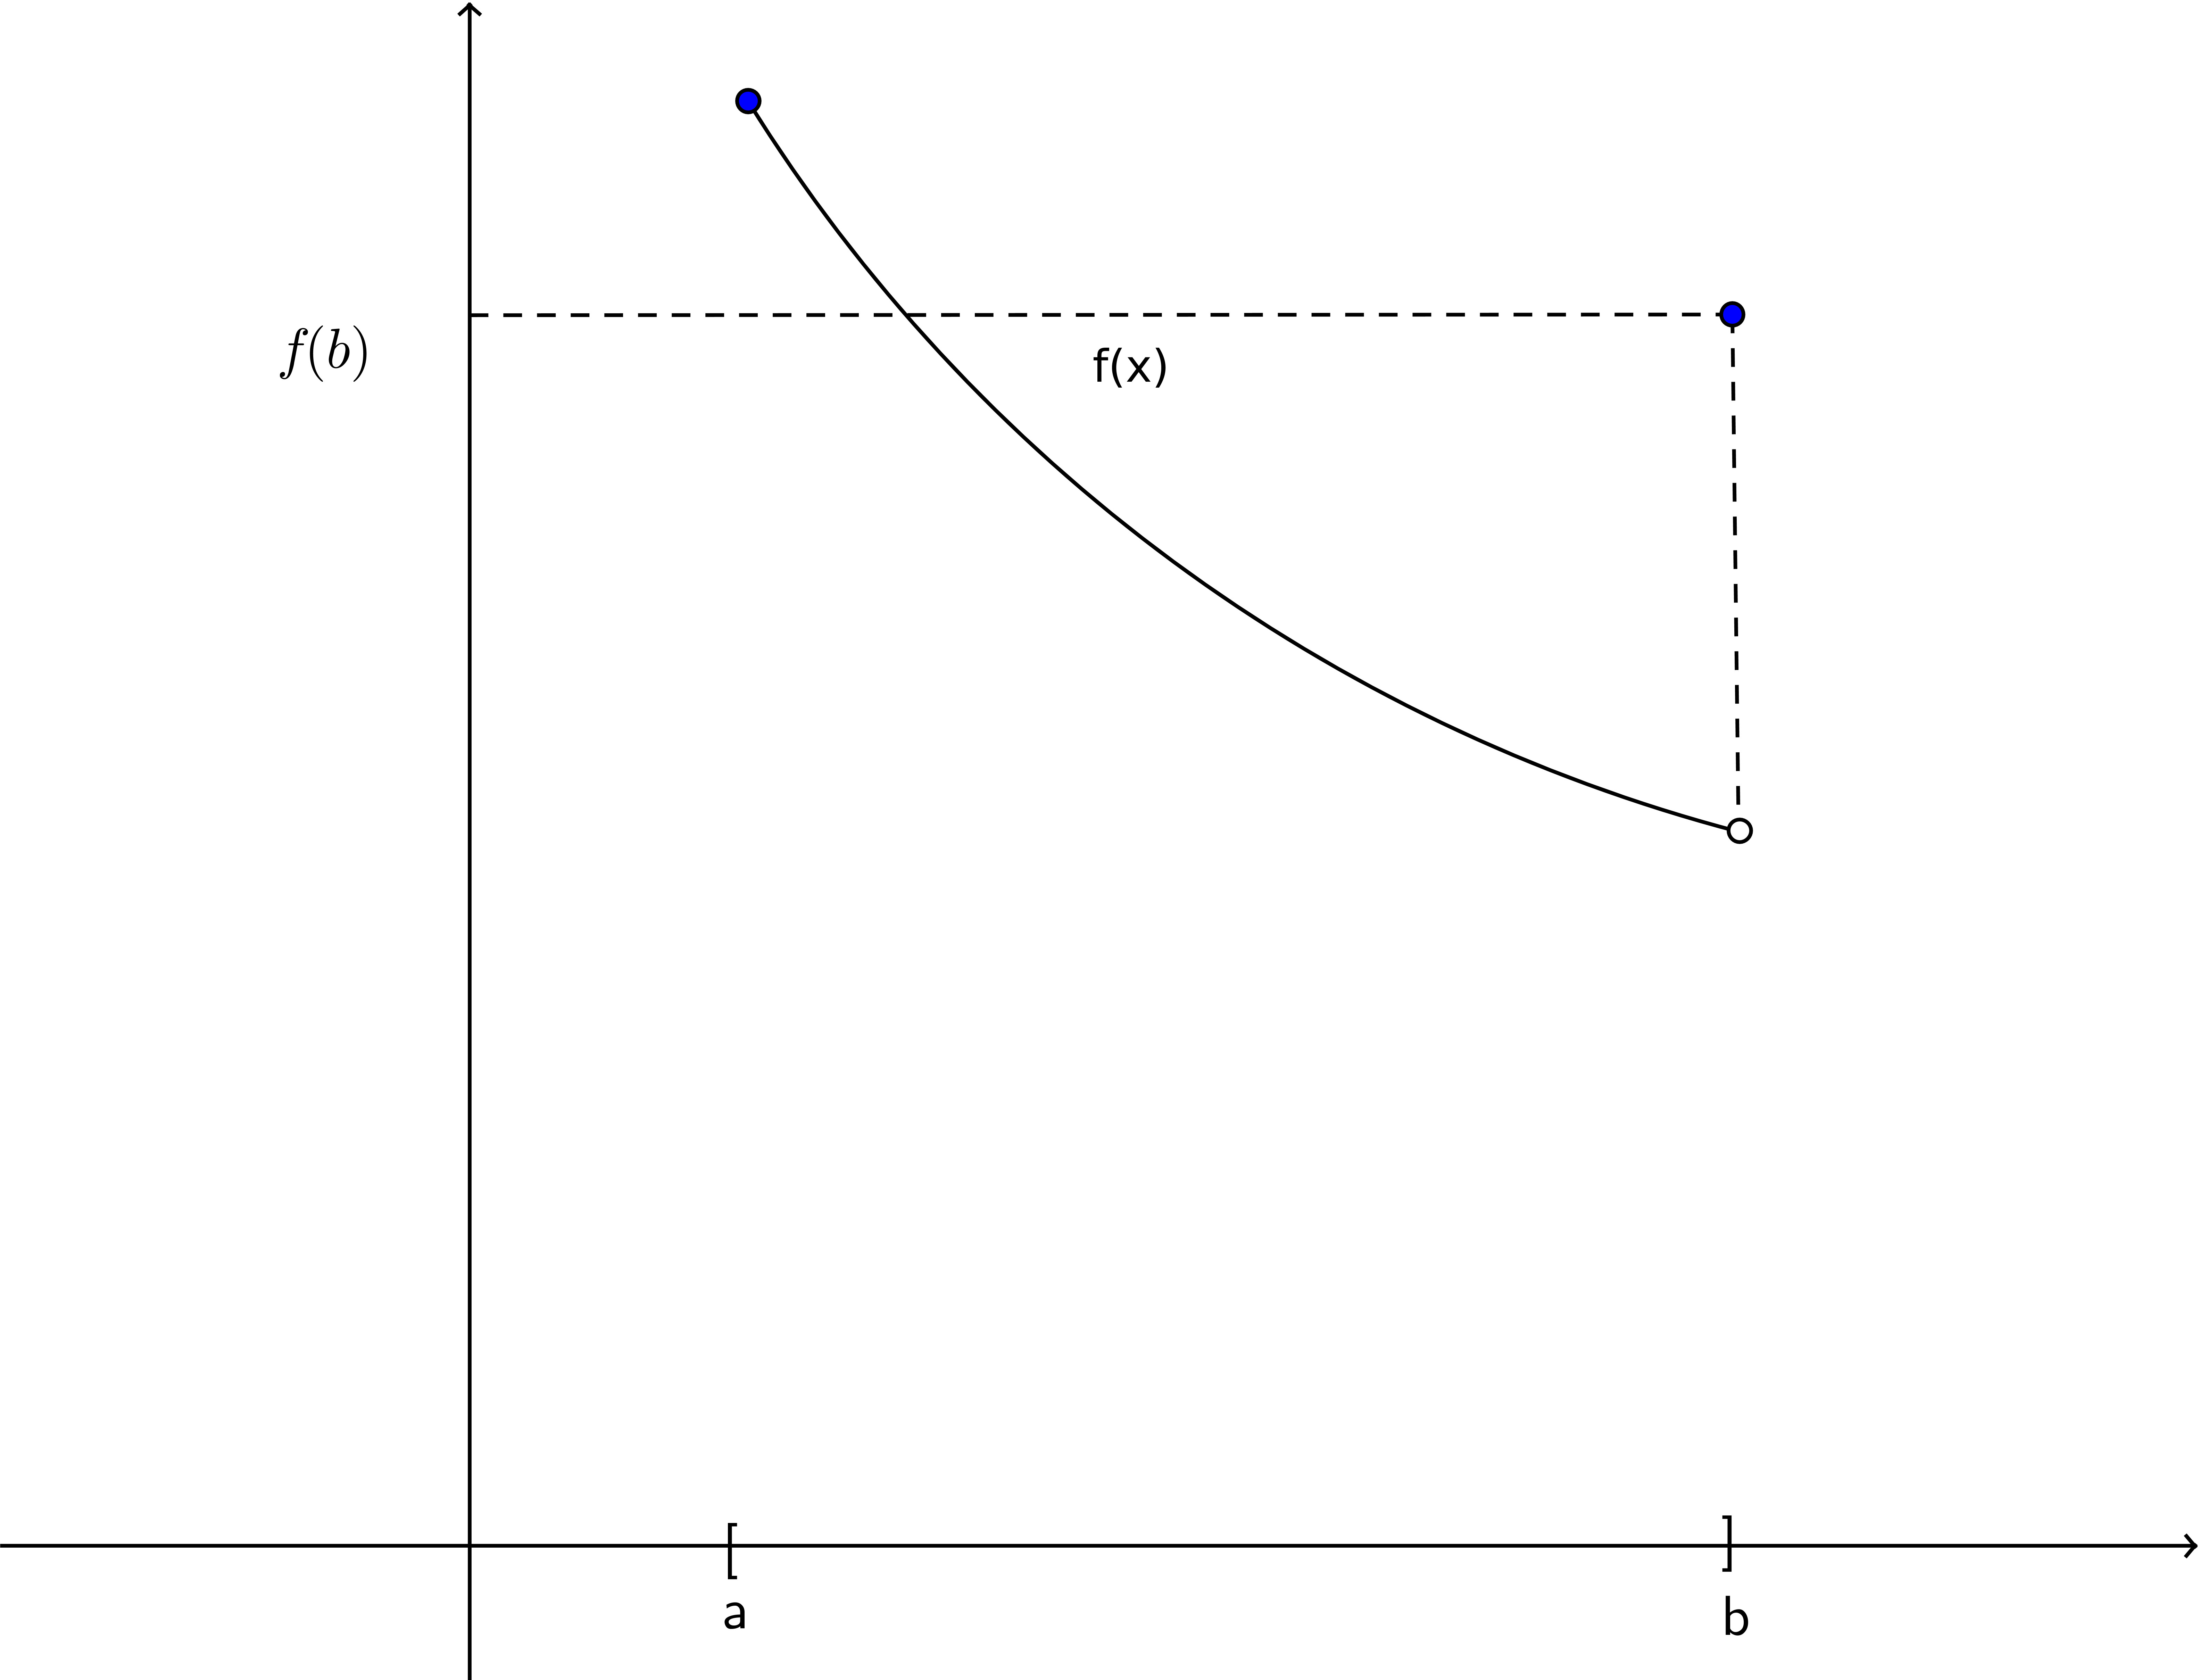
\includegraphics[scale = 0.1]{./partes/sub_sec/2_5b.jpg}}
   \subfigure[$f$ no acotada]{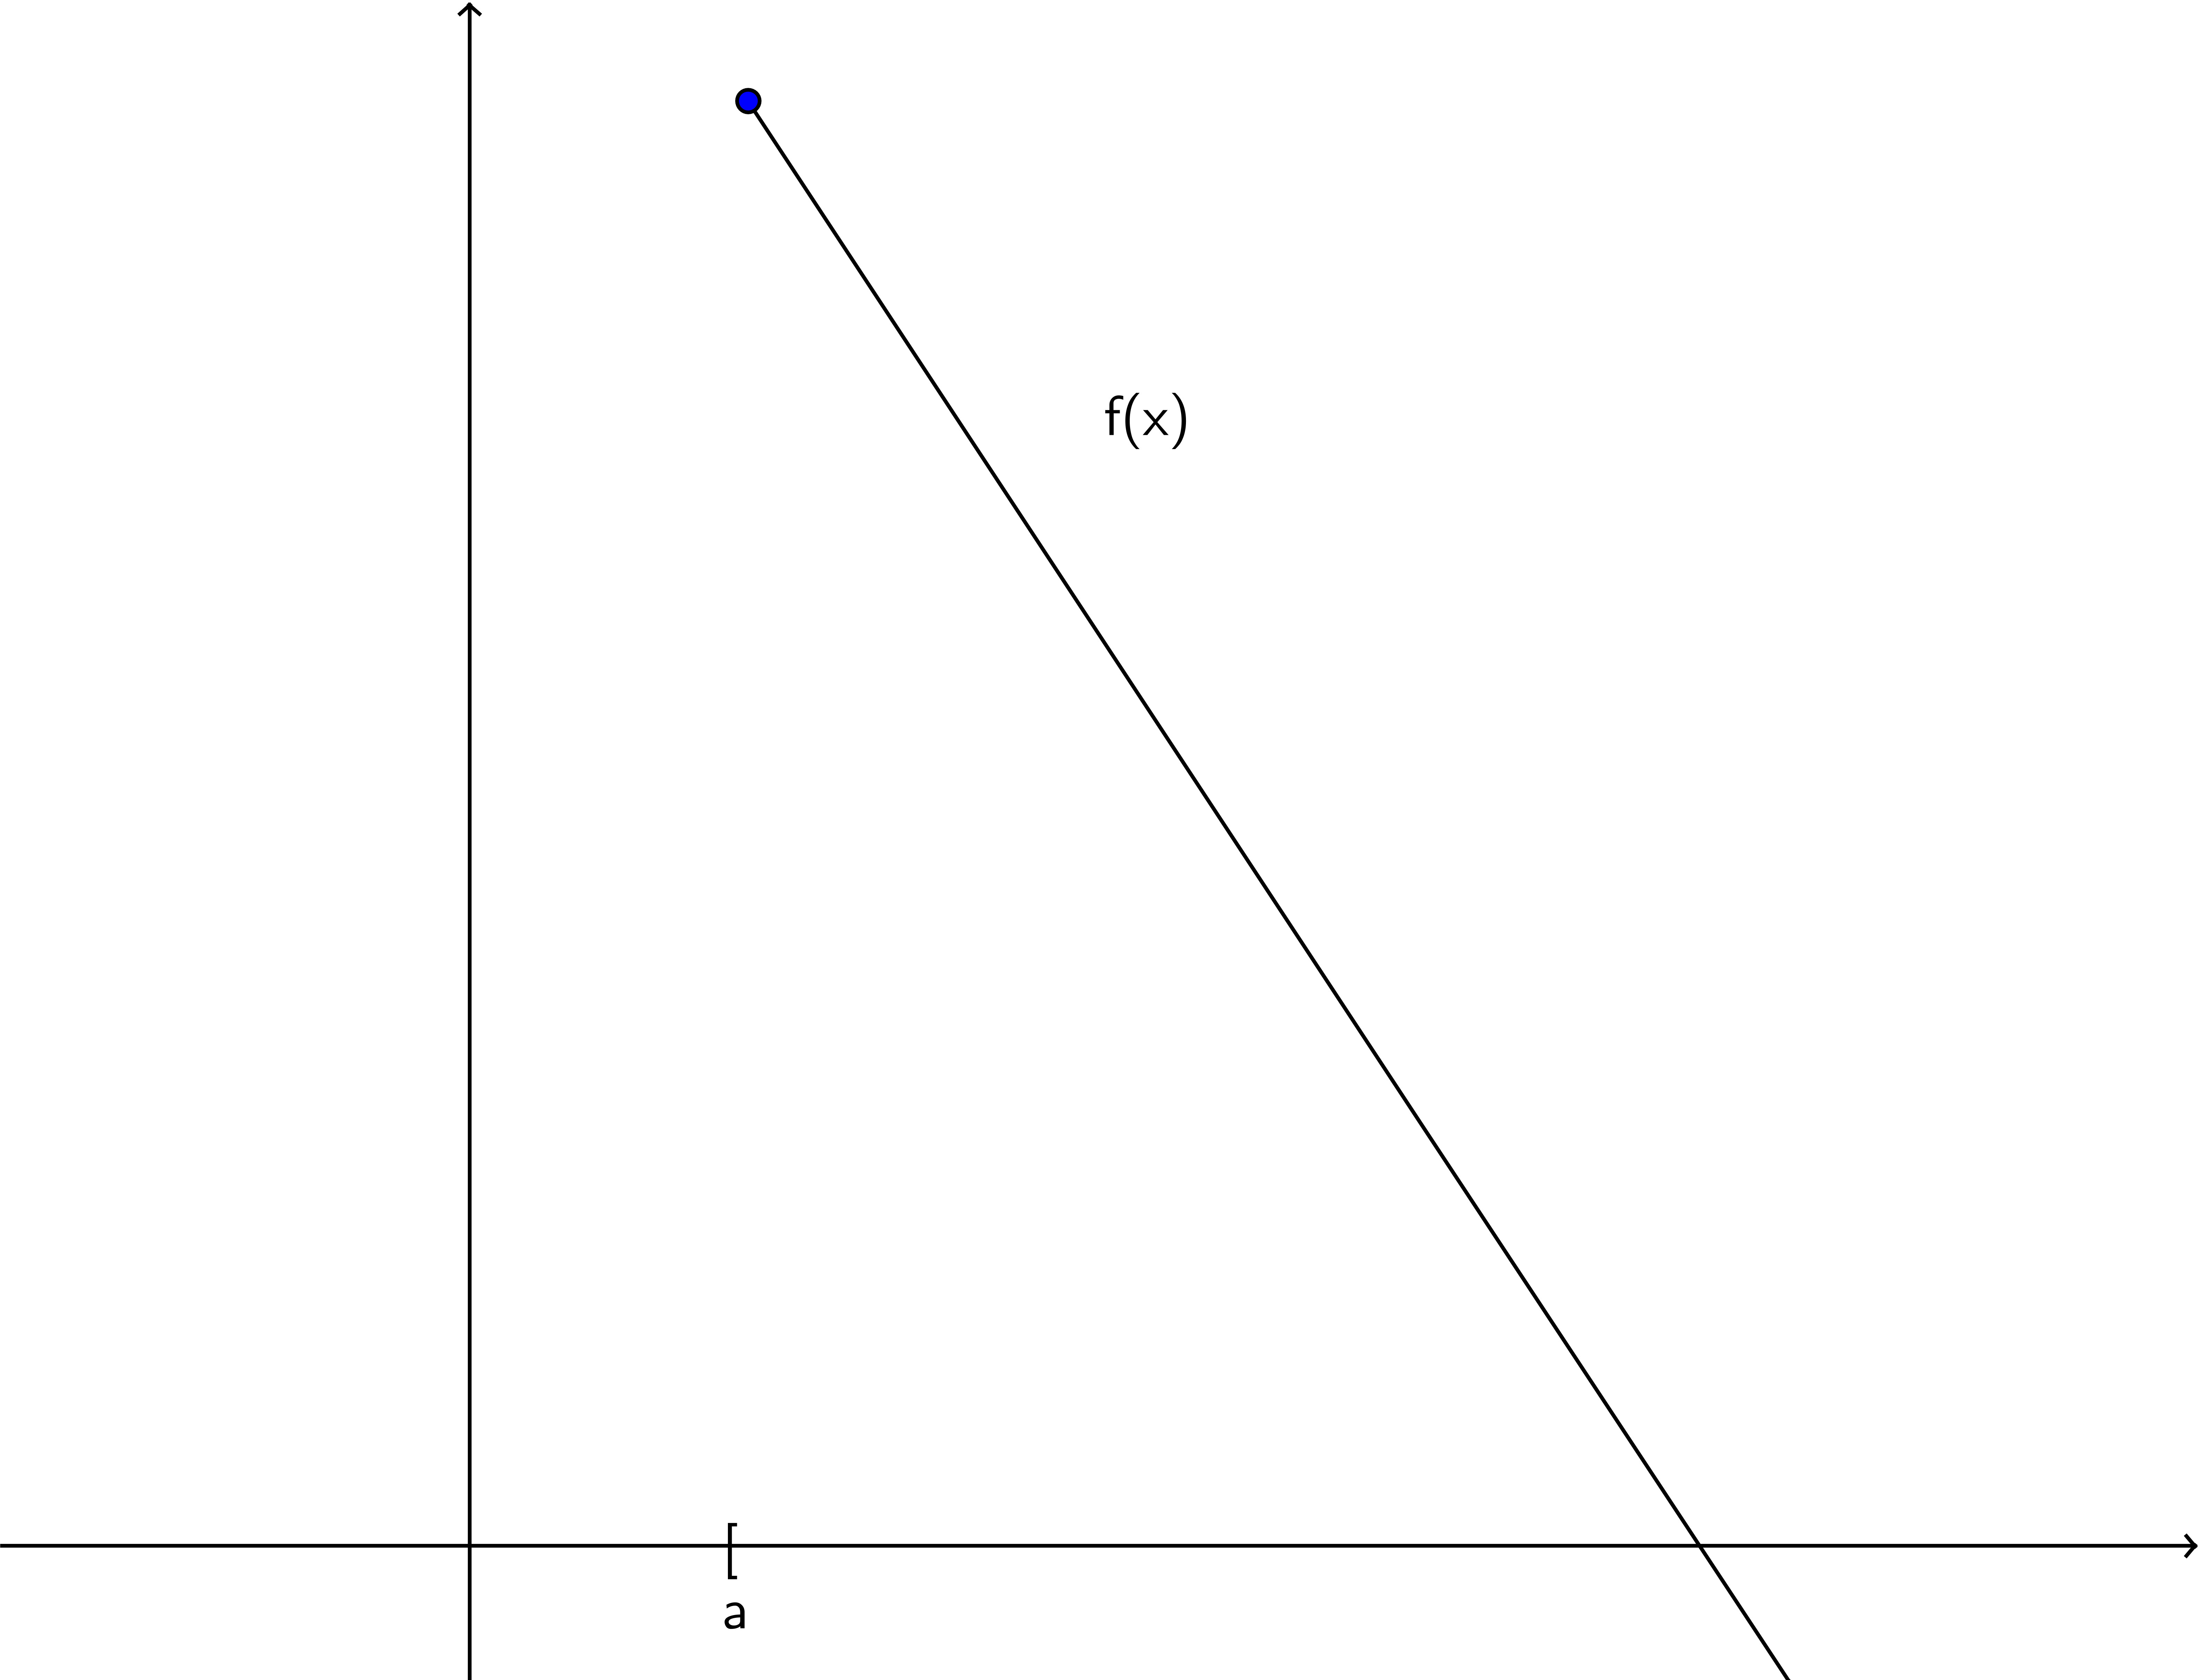
\includegraphics[scale = 0.1]{./partes/sub_sec/2_5c.jpg}}
   \caption{Inexistencia de soluci\'on de minimizaci\'on \cite{no-lineal}}
   \label{no_sol}
\end{figure}

%---------------------------------------------------------------------------------------

Ahora probaremos formalmente este resultado cuando $S$ es no vaci\'o, cerrado y acotado, $f$ continua en $S$, con \'estas condiciones
el m\'inimo en la Figura \ref{no_sol} si existe.\\

{\teorema Sea $S$ un conjunto no vac\'io, compacto y sea $f \longmapsto \mathbb{R}$ continua en $S$ entonces el problema
$\min \{f(x): x \in S\}$ alcanza su m\'inimo; esto es, existe una solucion de minimizaci\'on para este problema. \label{sol-min}}\\

\textbf{\itshape Demostraci\'on:}\\

Como $f$ es continua en $S$ y $S$ es cerrado y acotado, $f$ tambi\'en est\'a acotada (recordar que $f$ es continua), como $S \neq \emptyset$,
existe una cota inferior (la m\'as grande) $\alpha \equiv \min \{f(x):\, x \in S\}$. Ahora, sea $0 < \varepsilon < 1$ y consideremos el
conjunto $S_{k} = \{x \in S:\, \alpha \leqslant f(x) \leqslant \alpha + \varepsilon^{k}\}\,\, \forall\, k=1,\, 2, \ldots .$ Por la 
definici\'on de m\'inimo se tiene que $S_{k} \neq \emptyset \,\,\, \forall \, k$, entonces, tambi\'en podemos construir una sucesi\'on de puntos
$\{x_k\} \subseteq S$ seleccionando un punto $x_k \in S_k\,\, \forall \, k =1,\,2, \ldots $ Como $S$ es acotado, existe existe una
subseci\'on convergente $\{x_k \}_{K}\rightarrow \overline{x}$ indexada por el conjunto $K$. Por la cerradura de $S$ tenemos
$\overline{x} \in S$; y por la continuidad $f$ se tiene que como  $\alpha \leqslant f(x) \leqslant \alpha + \varepsilon^{k} \,\, \forall\, k$
tenemos que:

$$\alpha = \displaystyle{\lim_{k \rightarrow \infty; \,\, k \in K}} f(x_k) = f(\overline{x})$$

Por lo tanto, hemos demostrado que existe una soluci\'on $\overline{x} \in S$ tal que $f(\overline{x}) = \alpha = \inf \{f(x):\, x \in S\}$, 
entonces $\overline{x}$ es una soluci\'on de minimizaci\'on.
\begin{flushright}
   $\square$
\end{flushright}
%---------------------------------------fin de teorema de weistrass------------------------------------------------------------------------

\subsubsection{Separaci\'on y soporte de conjuntos}
\medskip

Las nociones de hiperplano soporte y separaci\'on de conjuntos convexos son muy importantes en optimizaci\'on. Casi todas las condiciones de
optimalidad y dualidad se relacionan con alg\'un tipo de separaci\'on o soporte de conjuntos convexos \cite{no-lineal}. Los resultados que veremos 
acontinuaci\'on est\'an basados en el siguiente hecho geom\'etrico: Dado un conjunto cerrado $S$  y un punto $y \in S$ existe un \'unico punto
$\overline{x} \in S$ con con una distancia m\'inima a $y$ y un hiperplano que separa a $y$ y $S$.\\

\textbf{Distancia m\'inima de un punto a un conjunto convexo \cite{no-lineal}}\\
\\

Para establecer el importante resultado anterior seguiremos la {\it ley del paralelogramo}.\\
Sean $a$ y $b$ dos vectores en $\mathbb{R}^n.$ Entonces: 

\begin{eqnarray*}
   \parallel \vec{a} + \vec{b} \parallel ^2 &=& \parallel \vec{a} \parallel ^2 + \parallel \vec{b} \parallel ^2 + \,2 \vec{a^t} \vec{b} \\
   \parallel \vec{a} - \vec{b} \parallel ^2 &=& \parallel \vec{a} \parallel ^2 + \parallel \vec{b} \parallel ^2 - 2 \, \vec{a^t} \vec{b}
\end{eqnarray*}

Sumando ambas se tiene:
 \[\parallel \vec{a} + \vec{b} \parallel ^2 + \parallel \vec{a} - \vec{b} \parallel ^2 = 
2 \parallel \vec{a} \parallel ^2 + 2 \parallel \vec{b} \parallel ^2\]

Este resultado se ilustra en la Figura (\ref{paralelogramo}) y puede ser representado de la siguiente manera:
La suma de las normas al cuadrado de las diagonales de un paralelogramo es igual al doble de la suma de sus normas al cuadrado.

\begin{figure}   \centering
   
\definecolor{ffzzzz}{rgb}{1,0.6,0.6}
\begin{tikzpicture}[line cap=round,line join=round,>=triangle 45,x=1.0cm,y=1.0cm]
\clip(0.16,0.49) rectangle (5.74,3.4);
\fill[color=ffzzzz,fill=ffzzzz,fill opacity=0.1] (2,3) -- (0.52,1) -- (4.18,0.98) -- (5.28,3) -- cycle;
\draw [color=ffzzzz] (2,3)-- (0.52,1);
\draw [color=ffzzzz] (0.52,1)-- (4.18,0.98);
\draw [color=ffzzzz] (4.18,0.98)-- (5.28,3);
\draw [color=ffzzzz] (5.28,3)-- (2,3);
\draw [->] (0.52,1) -- (4.18,0.98);
\draw [->] (4.18,0.98) -- (5.28,3);
\draw [->] (0.52,1) -- (5.28,3);
\draw [->] (4.18,0.98) -- (2,3);
\draw (4.77,2.05) node[anchor=north west] {$a$};
\draw (2.19,1.05) node[anchor=north west] {$b$};
\draw (1.27,2.07) node[anchor=north west] {$a + b$};
\draw (2.54,3.05) node[anchor=north west] {$a - b$};
\end{tikzpicture}
   \caption{Ley del paralelogramo}\label{paralelogramo}
\end{figure} 

%--------------------------------------------separacioon de hiperplanos--------------------------------------
De la teor\'ia b\'asica de geometr\'ia en espacios vectoriales normados se tiene que un hiperplano cerrado $H$ en $X$ puede ser reperesentado
por: \cite{pajardo}

$$H= \{ x \in X: \langle x, x^* \rangle = \alpha \}$$

Para alg\'un $x^* \in X*$ y $\alpha \in \mathbb{R}$. De igual modo un semiespacio cerrado $\mathcal{H}$ de $X$ puede ser representado por:

$$\mathcal{H} = \{x \in X: \langle x, x^*\rangle \leqslant \alpha \}$$

Para alg\'un $x^* \in X^*$ y $\alpha \in \mathbb{R}$.\\ \\


{\teorema Sea $C \subset X$ un conjunto convexo cerrado no vac\'io del espacio vectorial normado $X$.
Entonces, cada elemento $ u \notin C$ puede ser fuertemente separado de $C$ por un hiperplano 
cerrado, es decir,

$$\exists \, z^* \in X^*, \, z^* \neq 0,\,\, \exists \alpha \in \mathbb{R}\,\, \mbox{tal que} \,\,
\langle u, z^* \rangle > \alpha \,\, \mbox{y}\,\, \langle x, z^* \rangle \leqslant \alpha \,\, 
\forall  x \,\in \, C$$
\label{separacion} }\\ 

Para la demostracion del teorema es necesario conocer los resultados del teorema de Hanh-Banach, el 
cual dice:

{\teorema: {\bf(Primera forma geom\'etrica del Teorema de Hahn-Banach)} \\
Sean $A \subset C \, \mbox{y} \,\, B\subset C$ subconjuntos convexos no vac\'ios tales que $A \cap B = 
\emptyset.$ Supongamos que uno de ellos es abierto. Entonces existe un hiperplano cerrado que separa
$A \,\, \mbox{y} \,\, B.$ \label{hb1}}

{\teorema: {\bf(Segunda forma geom\'etrica del teorema de Hahn-Banach)}\\
Sean $A \subset C \, \mbox{y} \,\, B\subset C$ subconjuntos convexos no vac\'ios tales que $A \cap B = 
\emptyset.$ Supongamos que $A$ es cerrado y $B$ es compacto. Entonces existe un hiperplano cerrado
que separa estrictamente $A \,\, \mbox{y} \,\, B.$  \label{hb2} }\\ \\
\

\textbf{Demostraci\'on: (Teorema \ref{separacion})}\\
La demostraci\'on est\'a dada cuando el espacio vectorial $X$ es un espacio de Hilbert. Para 
el caso general, se utiliza la versi\'on anal\'itica del teorema de Hahn-Banach el cual es una 
consecuencia del lema de Zorn.
\medskip

Recordemos que si $X$ es un espacio de Hilbert, entonces $X^*$ se identifica con $X$ y se tiene que
$\parallel x \parallel^2 = \langle x, x \rangle$ (producto interno "$=$" producto de dualidad).\\ 
\ 
Sea Proy$_c (u)$ la proyecci\'on de $u \in X$ sobre el conjunto $C$ (\'esta existe y es \'unica). 
Proy$_c (u)$ est\'a caracterizada por 

\[\left\{ \begin{array}{rcl}
            \langle u - \mbox{Proy}_c (u), x -  \mbox{Proy}_c (u) \rangle & \leqslant & 0,\,\,
            \forall \, x  \in C\\
            \mbox{Proy}_c (u)   & \in & C
          \end{array}
\right. \]
\\ 
\
Por otro lado 

\begin{eqnarray}
      0 < \parallel z^*\parallel^2 & = & \langle z^*, \,\,z^* \rangle \nonumber \\
      & = &  \langle u, \,\,z^* \rangle - \langle \mbox{Proy}_{C}(u), \,\,z^* \rangle \\
      & \Longrightarrow & \langle u, \,\, z \rangle > \langle \mbox{Proy}_{C}(u), \,\,z^* \rangle
\end{eqnarray}

Tomemos $\alpha:= \langle z, \,\, \mbox{Proy}_{C}(u) \rangle.$\, Combinando (2) y (3) se obtiene:
\[ \sup_{x\, \in \, C} \langle x, \, z^*  \rangle  \leqslant \alpha < \langle u, \, z^{*} \rangle\]

Lo cual demuestra el resultado. \begin{flushright}
                                   $\square$
                                \end{flushright}

%----------------------------------fin de separacion de hiperplanos---------------------------------
%Preguntar, hasta donde llegamos con separacion de espacios por hiperplanos














